\scanpage{57}
\deleted{is \unsure{determined|determined} by the graph structure with a vertex \unsure{weighted|weighted} \unsure{by the}}

The simplest cases are the elementary cases (\inserted{one-point} graphs \deleted{with \unsure{one isolated point}})
\margin{Elementary MD-graphs (isolated vertex \inserted{i.e. zero modular codimension}) of modular dimension $1$ \deleted{\illegible{1}} \deleted{\unsure{of dimension|ambient}\ $1$}}
\figure{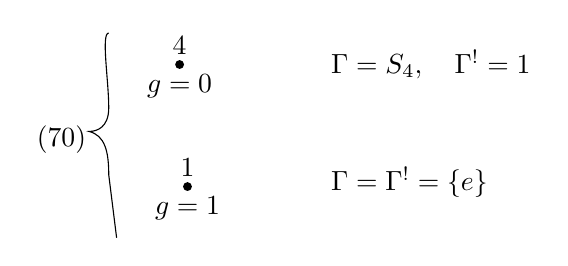
\begin{tikzpicture}[x=1cm,y=1cm]
\node at (-1.3,-.75) {$(70)$};\draw (-.7,.6) .. controls (-.8,.6) and (-.7,0) .. (-.7,-.35) .. controls (-.7,-.6) and (-.85,-.65) .. (-.95,-.65) .. controls (-.75,-.7) and (-.7,-.9) .. (-.7,-1.2) -- (-.6,-2);
\fill (.2,.2) circle(1.6pt);\node[above] at (.2,.2) {$4$};\node[below] at (.2,.2) {$g=0$};\node[right] at (2,.2) {$\Gamma=\mathfrak S_4,\quad\Gamma^!=1$};
\fill (.3,-1.35) circle(1.6pt);\node[above] at (.3,-1.35) {$1$};\node[below] at (.3,-1.35) {$g=1$};\node[right] at (2,-1.3) {$\Gamma=\Gamma^!=\{e\}$};
\end{tikzpicture}}
The other cases are those of the ``\uline{\unsure{rational|retro-null}}'' \inserted{MD-}graphs (all the $g_\alpha$ zero) such that all the $\widehat\nu_\alpha$ are equal to three (thus the vertices of order $1\leq\widetilde\mu_\alpha\leq3$) \deleted{\unsure{and one}} \inserted{except }one of them, which is equal to $4$ (thus $1\leq\widetilde\mu_{\alpha_0}\leq4$), or else of \inserted{MD-}graphs which have all their vertices except one rational and $\widehat\nu_\alpha=3$, \deleted{(thus} except one \inserted{$\alpha_0$} which is an end-vertex ($\widetilde\mu_\alpha=1$) and of genus $1$, $\nu_{\alpha_0}=0$ --- thus here all the vertices are of order $1\leq\widetilde\mu_\alpha\leq3$, and the $\nu_\alpha$ \inserted{for $\alpha\ne\alpha_0$} are equal to $3-\widetilde\mu_\alpha$, \deleted{for $\alpha\ne$} and $\nu_{\alpha_0}=0$.

In both cases \inserted{($g_{\alpha_0}=0$, $\unsure{g_{\alpha_0}|g_\alpha}=1$)} we shall have a canonical isomorphism of multiplicities
\[
\text{(71)}\qquad\widehat M_G\simeq\widehat M_{g_{\alpha_0},\widehat I_{\alpha_0}}
\]
\margin{with $\widehat I_{\alpha_0}=I_{\alpha_0}+\widetilde A_{\alpha_0}$ (of cardinality $4$ or $1$, according as $g_{\alpha_0}=0$ or $g_{\alpha_0}=1$)}
\margin{56}
